\documentclass[../main.tex]{subfiles}
\begin{document}

\chapter{里德堡原子阵列中的量子多体疤痕}

\section{引言与理论背景}
在此背景下,一个引人注目的前沿是动力学受限系统内的量子信息动力学,例如里德堡原子阵列\cite{kumar2018sorting,sheng2022defect,graham2022multi,barnes2022assembly,kim2022rydberg,okuno2022high,chen2023continuous,liu2023realization,singh2023mid,eckner2023realizing,ma2023high,zhao2023floquet,bluvstein2024logical,gregory2024second,pause2024supercharged,shaw2024benchmarking}。
里德堡原子之间的强范德瓦尔斯相互作用导致里德堡阻塞机制\cite{lukin2001dipole,urban2009observation_combined},并约束局域量子比特翻转。这一基本物理过程可以由 PXP 哈密顿量近似描述\cite{lesanovsky2012interacting,turner2018weak}:
\begin{equation}
  \hat{H}_\text{PXP} =
  \sum_i\hat{P}_i\hat\sigma^x_{i+1}\hat{P}_{i+2}.\label{Eq:PXP}
\end{equation}
这里,$\hat{P}_i = (1 - \hat\sigma^z_i)/2$ 是格点 $i$ 处自旋向下 $\ket{\downarrow}$ 态的投影算符,$\hat\sigma^{x,y,z}_i$ 是第 $i$ 个自旋的泡利矩阵。先前对这些系统的研究揭示了量子多体疤痕\cite{bernien2017probing,turner2018weak,serbyn2021quantum,bluvstein2021controlling, desaules2024ergodicity}。此外,最近的理论研究\cite{yuan2022quantum}表明,动力学受限多体系统,如 PXP 模型描述的系统,可能蕴藏着尚未发现的信息加扰机制,为探索超越多体疤痕范围的独特时空量子信息动力学开辟了新前沿。

图~\ref{Fig:1}a 描绘了对这种动力学受限系统中新颖信息传播动力学的直观理解。在 PXP 模型中,翻转反铁磁奈尔态
$\ket{\mathbb{Z}_2}=
 \ket{\uparrow\downarrow\uparrow\downarrow\uparrow\cdots}
$
中的中心自旋编码了一比特信息。这种局域微扰诱导了相邻自旋旋转的迟滞,然后弹道式传播,形成线性光锥状波前。在这个光锥内,自旋恢复其受限旋转,但自旋态的可分辨性周期性地消失和重现,这由它们 $\hat\sigma^y$ 期望值的差异(虚线圆圈)所标志。这种行为与典型的混沌量子系统显著不同,在后者中,光锥内的自旋态由于加扰而迅速变得不可分辨。
这些动力学受限动力学可能导致持续的信息回流和量子混沌的不寻常破坏,暗示了探测独特信息加扰动力学的新途径\cite{yuan2022quantum}。

\section{材料与方法:实验装置与控制}

\subsection{实验方法概述}

\subsubsection{无缺陷原子阵列的制备}
在本文的实验中,原子从磁光阱加载并被通过空间光调制器 (SLM) 衍射的聚焦 808-\unit{nm} 激光束形成的光镊捕获。测量和反馈过程消除了原子链中的缺陷,实现了全填充阵列的快速创建(图~\ref{Fig:extended_1}a)。

\subsubsection{实验参数}
一旦制备好无缺陷阵列,所有原子都被光泵浦到基态。原子间距约为 \SI{7}{\micro m},导致最近邻和次近邻相互作用分别为 $V_{i,i+1} = 2\pi \times \SI{7.3}{MHz}$ 和 $V_{i,i+2} = 2\pi \times \SI{0.11}{MHz}$。为了尽管 vdW 相互作用 $V_{i,i+1} / V_{i,i+2}$ 的固定比率为 64 仍能紧密近似 PXP 模型,基态-里德堡驱动拉比频率 $\Omega$ 在态演化期间设置为 $V_{i,i+1}/6 = 2\pi \times \SI{1.21(1)}{\MHz}$,在两个相互作用强度之间取得平衡。此外,引入小的失谐 $\Delta =2\pi\times\SI{0.22(1)}{\MHz}$ 以补偿残留的次近邻里德堡相互作用 $V_{i,i+2}$。
在这些实验参数下,实验里德堡哈密顿量可以被 PXP 模型很好地近似,数值模拟显示偏差可忽略不计(详见第~\ref{section:experimental-parameter} 节)。

\subsubsection{高保真度 $\ket{\mathbb{Z}_2}$ 态制备}
795-\unit{\nano\meter} 和 480-\unit{\nano\meter} 寻址激光束通过 SLM 衍射产生,并通过高数值孔径物镜聚焦到原子上,通过调整 SLM 相位图案实现选择性寻址。795-\unit{\nano\meter} 寻址光束非共振地耦合 $\ket{5S_{1/2}}$ 基态到 $\ket{5P_{1/2}}$ 态(图~\ref{Fig:extended_1}b),在被寻址原子上诱导光频移。在 $\ket{\mathbb{Z}_2}$ 态制备期间,被寻址原子经历 $2\pi \times \SI{12.2(3)}{MHz}$ 的光频移,足以屏蔽原子免受里德堡激发。
结合高保真度全局 $\pi$ 脉冲,我们实现了多达 25 个原子阵列的高保真度制备(图~\ref{Fig:2}b)。

\begin{figure*}[!ht]
  \centering
  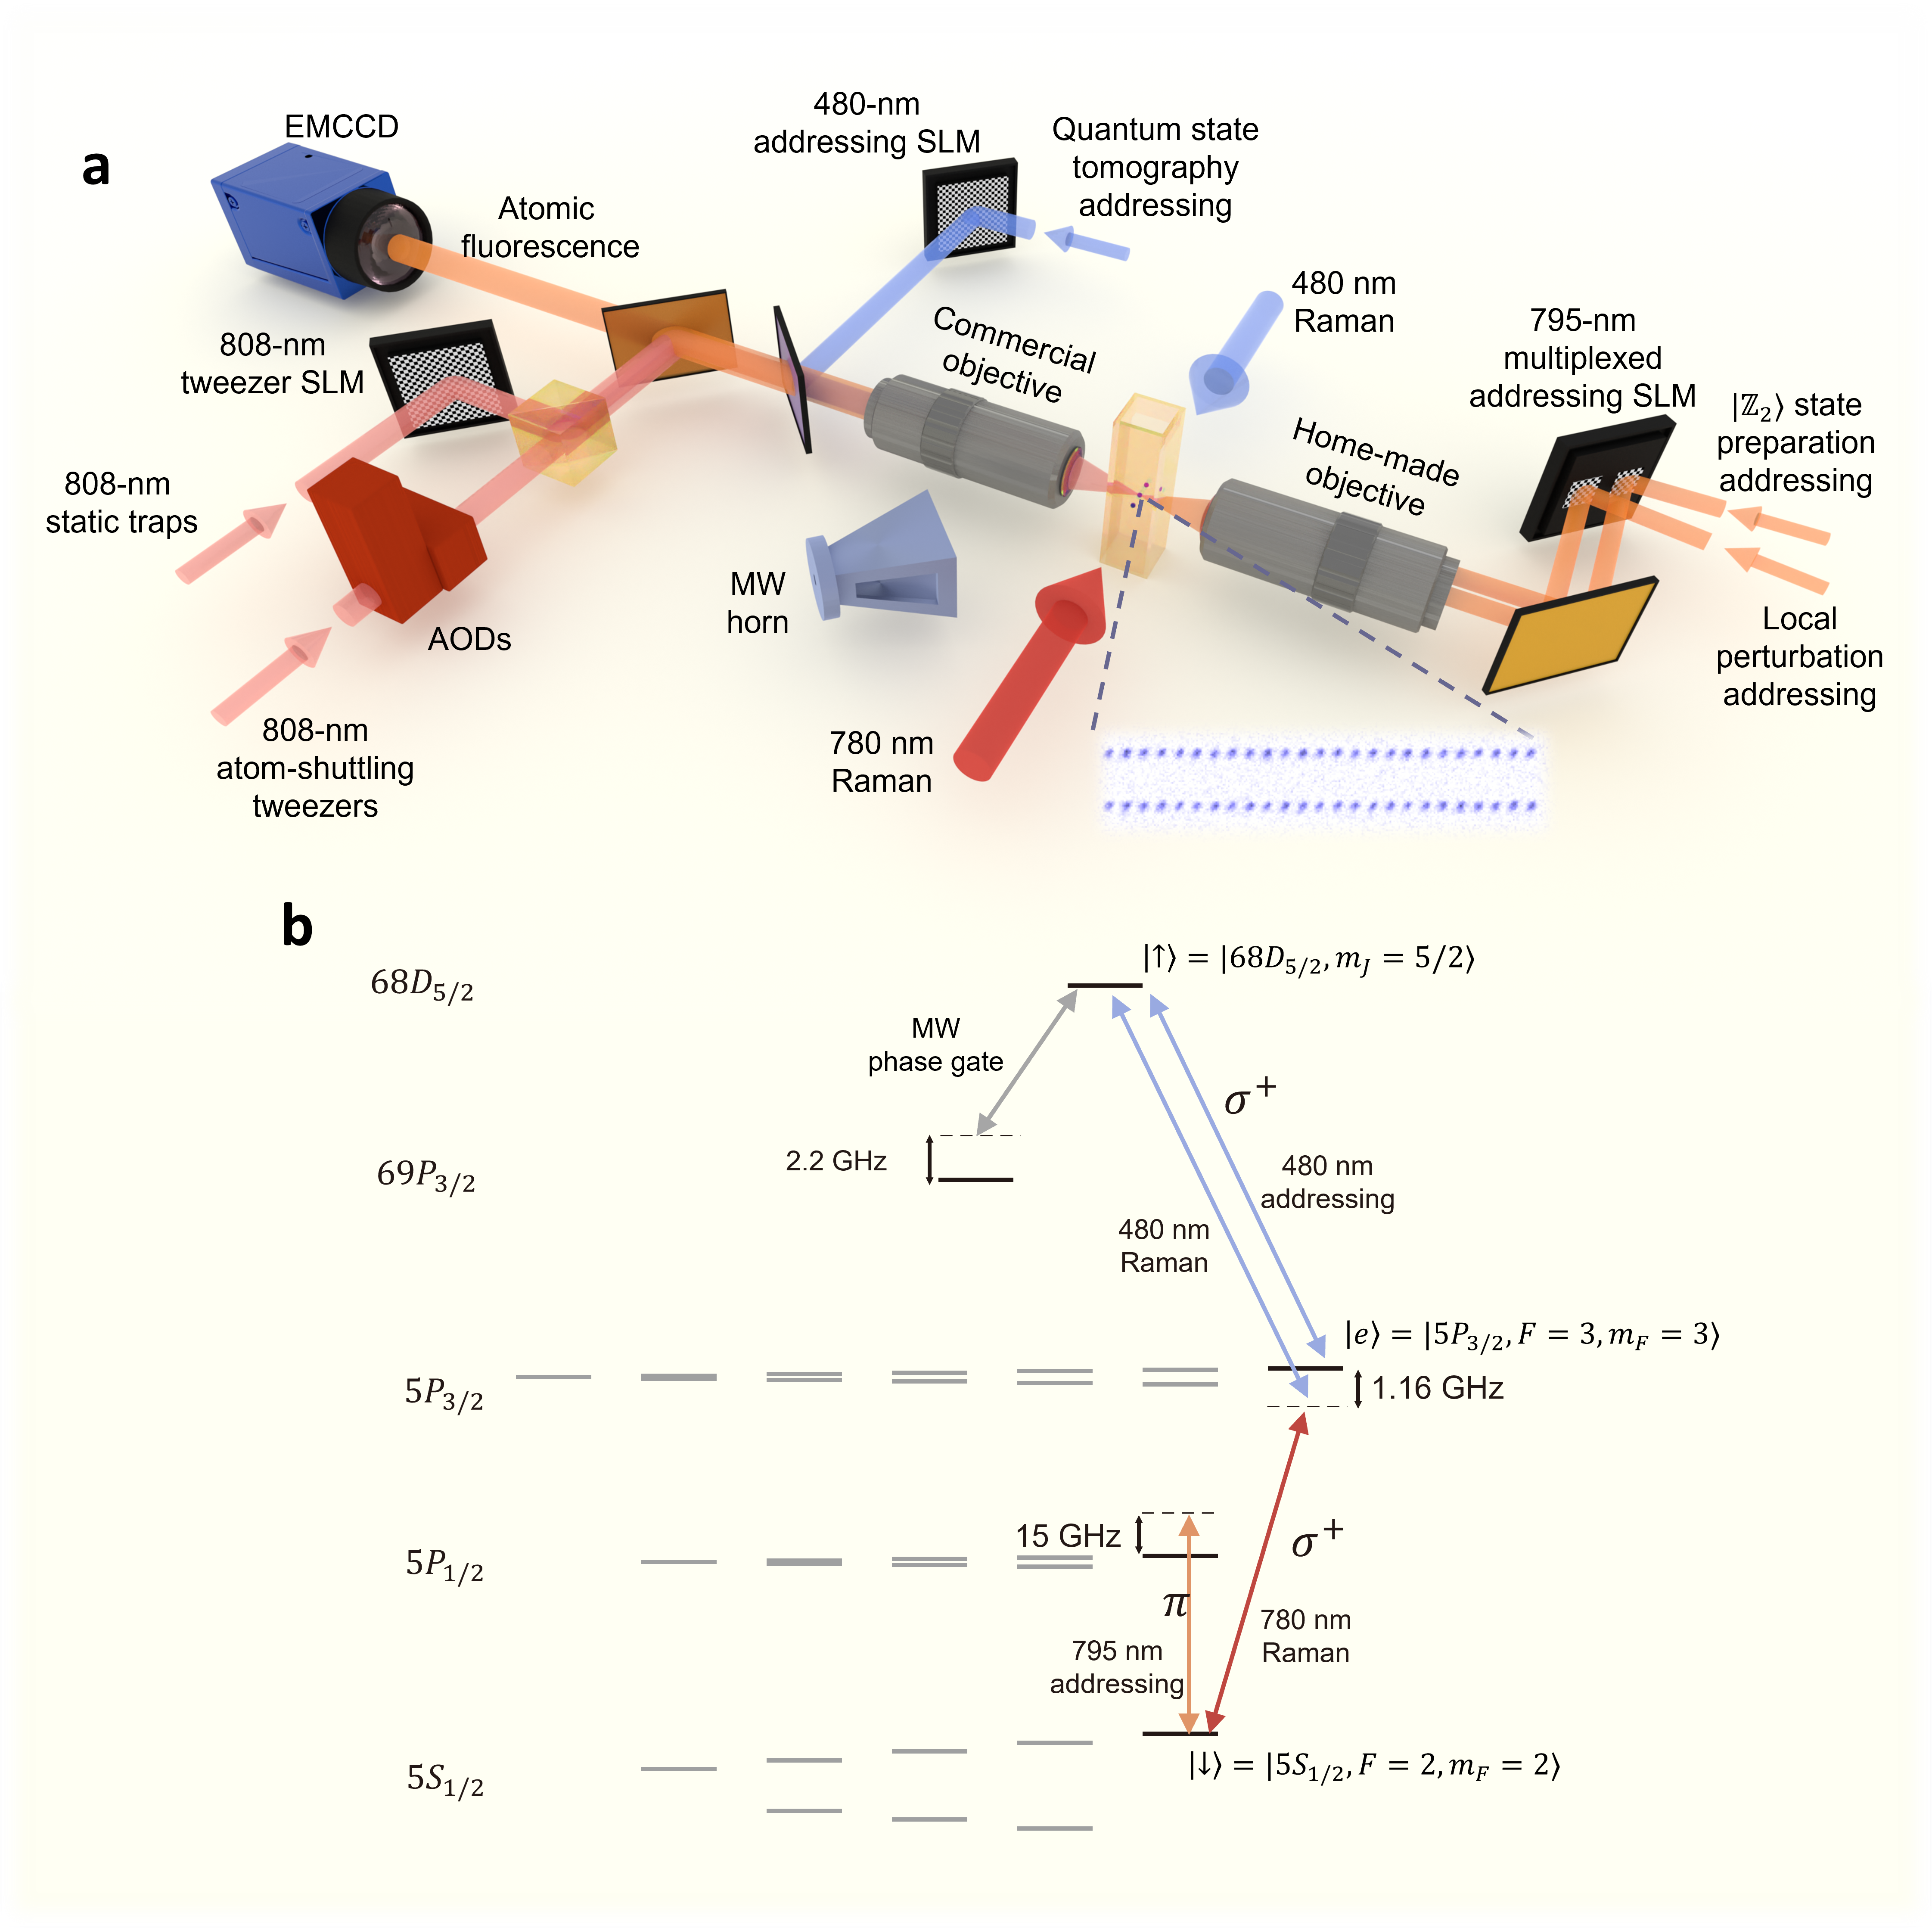
\includegraphics[width=0.7\textwidth]{chapters/chapter_06/figure/Extended_Fig_1.png}
  \caption{
    \textbf{实验装置和原子能级图。} 
    \textbf{a}, 实验装置中基本元件的示意图。808-nm 静态光镊由 SLM 产生,而原子运输光镊由两个声光偏转器 (AODs) 控制。480-\unit{\nano\meter} 寻址激光束由另一个 SLM 产生。商业物镜 (G Plan Apo 50$\times$, Mitutoyo, NA = 0.5) 聚焦 808-nm 光镊光束和 480-\unit{\nano\meter} 寻址光束,同时收集 795-\unit{\nano\meter} 原子荧光用于电子倍增 CCD (EMCCD) 相机上的成像。反向传播的 780-\unit{\nano\meter} 和 480-\unit{\nano\meter} 拉曼光束实现相干基态-里德堡操控。用于局域微扰 \(\hat\sigma_c^z\) 的 795-\unit{\nano\meter} 寻址激光和负责产生用于 $\ket{\mathbb{Z}_2}$ 态制备的交替光频移的激光阵列瞄准同一 SLM 的不同区域。这些不同区域显示不同的全息图,实现不同的寻址激光图案。这种空间复用技术允许在 \(\ket{\mathbb{Z}_2}\) 态制备和局域微扰激光配置之间进行亚微秒切换。795-\unit{\nano\meter} 寻址激光束通过自制物镜 (NA = 0.4) 聚焦到原子上。腔体附近的微波喇叭产生用于里德堡态操控(相位门)和探测的微波脉冲。插图显示了原子阵列。
    \textbf{b}, 显示实验中涉及的 $^{87}$Rb 原子能级的能级图。我们的里德堡激发方案采用从基态 \(\ket{\downarrow} = \ket{5S_{1/2}, F=2, m_F=2}\) 到里德堡态 \(\ket{\uparrow} = \ket{68D_{5/2}, m_J=5/2}\) 的双光子拉曼跃迁。该跃迁由 \(\hat\sigma^+\) 偏振的 780-\unit{\nano\meter} 激光(耦合基态到中间态 \(\ket{e}=\ket{5P_{3/2}, F=3, m_F=3}\))和 \(\hat\sigma^+\) 偏振的 480-\unit{\nano\meter} 激光(连接中间态到里德堡态)驱动。两束激光相对于中间态失谐 \(\Delta = 2\pi\times\SI{1.16}{\giga\hertz}\)。微波场相对于 \(\ket{\uparrow}\) 到 \(\ket{69P_{3/2}, m_J=3/2}\) 跃迁红失谐 $2\pi\times\SI{2.2}{\giga\hertz}$,在里德堡态上产生交流斯塔克频移,并提供用于反转 PXP 哈密顿量的相位门。对于局域单量子比特控制,采用相对于 \(\ket{\downarrow}\)-\(\ket{5P_{1/2}}\) 跃迁蓝失谐 $2\pi\times\SI{15}{\giga\hertz}$ 的 795-\unit{\nano\meter} 寻址光束,以及与 \(\ket{\uparrow}\)-\(\ket{e}\) 跃迁共振的 480-\unit{\nano\meter} 寻址光束。
    }
  \label{Fig:extended_1}
\end{figure*}

\section{实验细节}
\label{section:experiment}
{
可编程原子阵列已成为量子模拟和计算的新型平台,为探索量子多体现象提供了卓越的控制能力和可扩展性。
在过去十年中,该领域取得了显著进展,包括原子阵列的制备~\cite{piotrowicz2013two,endres2016atom,barredo2016atom,lee2017defect,barredo2018synthetic,kumar2018sorting,sheng2022defect,barnes2022assembly,okuno2022high,liu2023realization,pause2024supercharged},在量子计算~\cite{isenhower2010demonstration,jau2016entangling,sheng2018high,omran2019generation,guo2020balanced,bluvstein2022quantum,graham2022multi,fu2022high,schine2022long,singh2023mid,evered2023high,scholl2023erasure,ma2023high,zhao2023floquet,bluvstein2024logical,gregory2024second,shaw2024benchmarking}、量子优化~\cite{graham2022multi,ebadi2022quantum,kim2022rydberg,bluvstein2024logical}、量子模拟~\cite{bernien2017probing,keesling2019quantum,ebadi2021quantum,scholl2021quantum,semeghini2021probing,fang2024probing,DeLeseleuc2019,scholl2022microwave,chen2023continuous,kim2024realization}以及量子计量学~\cite{bornet2023scalable,eckner2023realizing}方面的努力。
本节介绍了我们实验的细节,包括实验装置、时序以及 $\ket{\mathbb{Z}_2}$ 态的制备和表征。
}



\subsection{实验装置}
\label{section:setup}

{
本文的实验平台建立在双腔真空系统周围,由 2D 磁光阱 (MOT) 腔和科学腔组成。在 2D-MOT 腔中,$^{87}$Rb 原子源(安瓿)产生扩散的原子蒸气。这些原子被磁场和 780-\SI{}{\nano\meter} 激光冷却和束缚,激光相对于 $\ket{5S_{1/2}, F=2} \rightarrow \ket{5P_{3/2}, F=3}$ 循环跃迁红失谐 $2\pi\times \SI{30}{\MHz}$。预冷的原子系综随后通过差分泵浦孔径由 780-\SI{}{\nano\meter} 推送光束转移到科学腔中。
科学腔是一个定制设计的具有大光学通道的长方体玻璃腔 (Japan Cell)。腔内的超高真空条件由非蒸散型吸气剂泵 (NEXTorr D 200-5, SAES) 维持,实现了远低于 \(10^{-11}\) mbar 的压力。这种低背景压力最初允许单原子捕获寿命超过 10 分钟。然而,由于 2D-MOT 腔中离子泵 (SP-4, JJJvac) 的故障,寿命已降至约 \SI{90} 秒。原子在科学腔中被三维磁光阱 (3D-MOT) 捕获和冷却,使用三对反向传播的 780-\SI{}{\nano\meter} 激光束,磁场梯度为 \SI{0.15}{\tesla\per\cm}。每束光包含相对于 \(\ket{5S_{1/2}, F=2} \rightarrow \ket{5P_{3/2}, F=3}\) 循环跃迁红失谐 $2\pi\times \SI{24}{\MHz}$ 的冷却光,以及与 \(\ket{5S_{1/2}, F=1} \rightarrow \ket{5P_{3/2}, F=2}\) 跃迁共振的再泵浦光。
}

{
单个原子被捕获在由 808-nm 激光器 (TA pro, Toptica) 在自由运行模式下产生的静态二维光镊阵列中。激光束照射加载了通过加权 Gerchberg-Saxton (WGS) 算法生成的相位全息图的相位控制空间光调制器 (SLM, HED 6010-NIR-080-C, Holoeye)。此外,一个原子运输光镊系统,利用与静态阵列相同的 808-nm 激光源但偏振正交,允许精确的原子重排。原子运输光镊由一对正交取向的声光偏转器 (AODs, DTSX-400-800.850, AA Opto-Electronic) 控制,由双通道任意波形发生器 (AWG, M4i.6631-x8, Spectrum) 生成的具有独立任意波形的射频驱动。
}

{高数值孔径物镜 (G Plan Apo 50$\times$, Mitutoyo, NA = 0.5) 聚焦静态和可移动光镊,同时收集原子荧光,荧光被引导到电子倍增 CCD (EMCCD, iXon Ultra 888, Andor) 相机进行探测。此外,用于局域里德堡控制的 480-\SI{}{\nano\meter} 光束,利用类似的基于 SLM 的方法,通过同一物镜聚焦(见图~5a)。这种用于捕获、寻址和荧光探测的共享配置增强了系统的稳定性。}
{
与 Mitutoyo 物镜相对的是一个数值孔径为 0.4 的自制物镜。CCD 相机对静态光镊阵列成像,该阵列由 36 \(\times\) 2 个光镊组成,间距为 \SI{7}{\um},束腰约为 \SI{0.9}{\um}。通过迭代反馈和调整,整个阵列的强度变化保持在 1\% 以下。对于 \(\ket{\mathbb{Z}_2}\) 态制备和局域微扰至关重要的 795-\SI{}{\nano\meter} 寻址激光束通过自制物镜聚焦。两束反向传播的激光束——一束在 \SI{780}{\nm},另一束在 \SI{480}{\nm}——实现全局基态-里德堡相干操控。位于科学腔附近的微波天线产生用于里德堡态操控和探测的微波脉冲。
}

{
实验装置集成了用于态制备、量子比特控制和探测的多个激光系统。780-\SI{}{\nano\meter} 激光系统,一个锥形放大器激光器 (TA Pro, Toptica),用于 MOT 冷却光束和里德堡激发方案中的拉曼光。其频率被稳定到精细度为 26,000 的超低膨胀参考腔 (SLS)。AWG 驱动针对调制带宽进行了优化的单次通过声光调制器 (AOM, SGT200-780-0.5TA-B),以动态调整脉冲频率和强度。
为了耦合 \(\ket{e} \rightarrow \ket{r}\) 跃迁,采用了 480-\SI{}{\nano\meter} 激光系统(倍频 TA-SHG Pro, Toptica),960-nm 种子激光器锁定到与 780-\SI{}{\nano\meter} 激光器相同的参考腔。由直接数字合成 (DDS, AD9910) 驱动的 AOM 控制 480-\SI{}{\nano\meter} 激光束,该光束经过强度稳定并在整个里德堡操作序列中保持开启。里德堡激发激光的快速上升和下降沿是使用电光调制器 (EOMs) 实现的,以进行精确的开关切换。
}

\begin{figure}
  \centering
  \includegraphics[width=\textwidth]{chapters/chapter_06/figure/SI_Timing_sequence.png}  
  \caption{
    \textbf{实验时序。} 
    如第~\hyperref[section:timing-sequence]{1.2} 节所述的典型实验序列总结。用于 OTOC 和 Holevo 信息测量的详细里德堡实验序列在图~\ref{SI_OTOC_sequence},\ref{SI_HI_sequence} 中提供。
    }
  \label{Fig:S1}
\end{figure}




\subsection{实验时序} 
\label{section:timing-sequence}



{
实验序列开始于在科学腔中制备冷原子系综。3D MOT 加载 \SI{200}{\ms},产生直径为 \SI{500}{\um}、温度为 \SI{150}{\micro\kelvin} 的原子云,通过飞行时间 (TOF) 膨胀测量。为了进一步降低温度,应用了偏振梯度冷却 (PGC)。该过程涉及快速关闭磁场梯度(在 \SI{500}{\us} 内),同时将冷却光失谐增加到约 $2\pi\times\SI{90}{\MHz}$ 并降低冷却和再泵浦激光的强度。结果,原子被进一步冷却至约 \SI{40}{\micro\kelvin}。
}
{
激光冷却的原子系综作为随机加载可编程原子阵列的库。对于随机加载,使用两束反向传播的 795-\SI{}{\nano\meter} 激光束实施 \(\Lambda\) 增强灰光学粘团 (\(\Lambda\)GM)。
随后应用针对阱内冷却优化的额外偏振梯度冷却 (PGC) 阶段。这种组合冷却方法导致单原子加载效率约为 80\%,在深度为 \SI{1}{\milli\kelvin} 的阱中平均原子温度为 \SI{15}{\micro\kelvin},这是使用释放-再捕获 (R\&R) 方法测量的。原子荧光探测利用用于 \(\Lambda\)GM 的相同 795-\SI{}{\nano\meter} 光束,在将光阱深度增加到 \SI{1.3}{\milli\kelvin} 后进行复用。通过仔细平衡加热和冷却速率,在 \SI{30}{\ms} 曝光时间内实现了超过 99.9\% 的探测保真度,同时保持每次探测的平均原子损失低于 1\%。使用 795-\SI{}{\nano\meter} 荧光成像最小化了来自强 780-\SI{}{\nano\meter} 光束的串扰,确保了准确的原子探测。
}

{
原子重排过程产生无缺陷的一维原子链。该过程开始于将可移动光镊的强度从零线性增加到静态阱深度的三倍,将原子从静态 SLM 生成的阱转移到可移动光镊。然后用含时波形驱动 AODs 以平均速度 \SI{100}{\um\per\ms} 运输原子,遵循正弦速度分布以确保平滑的加速和减速。重排序列是使用改进的匈牙利算法 \cite{lee2017defect} 确定的,逐列优化原子移动。为了最小化移动光镊扫过静态阱时不必要的原子损失和加热,光镊路径包括额外的段以绕过中间的阱。重排过程的所有 AOD 波形都是预先计算的,允许快速执行序列。重排后测量表明,在 \SI{1}{\milli\kelvin} 深的阱中,原子温度增加到约 \SI{50}{\micro\kelvin}。
}

{
对于相干里德堡激发,采用双光子拉曼方案。具有 \(\sigma^+\) 偏振的红失谐 780-\SI{}{\nano\meter} 激光将基态耦合到中间态 \(\ket{5P_{3/2}, F=3, m_F=3}\)(见图~5b)。准直的 780-\SI{}{\nano\meter} 激光被引导到原子上,束腰约为 \SI{300}{\um},最大拉比频率为 \(\sim 2\pi\times\SI{100}{\MHz}\)。同时,同样具有 \(\sigma^+\) 偏振的蓝失谐 480-\SI{}{\nano\meter} 激光将中间态连接到里德堡态 \(\ket{\uparrow} = \ket{68D_{5/2}, m_J=5/2}\)。480-\SI{}{\nano\meter} 激光聚焦到原子上,束腰为 \SI{13}{\um},最大拉比频率为 \(\sim 2\pi\times\SI{70}{\MHz}\)。两束激光相对于中间态失谐 \(\Delta = 2\pi\times\SI{1.16}{\GHz}\)。
整个实验过程中施加 \SI{30}{\gauss} 的偏置磁场。
图~\ref{SI_Block_Rabi}a(蓝色圆圈)展示了由 780-\SI{}{\nano\meter} 和 480-\SI{}{\nano\meter} 激光驱动的单个原子的高对比度基态-里德堡态拉比振荡。当两个原子位于里德堡阻塞区域内时,$\Omega \ll V$,双里德堡激发受到强烈抑制,如图~\ref{SI_Block_Rabi}a 中的黄色方块所示。图~\ref{SI_Block_Rabi}a 中的红色菱形显示,贝尔态 $\frac{1}{\sqrt{2}}(\ket{\downarrow}\ket{\uparrow}+\ket{\uparrow}\ket{\downarrow})$ 和基态 $\ket{\downarrow}\ket{\downarrow}$ 之间的拉比振荡增强了 \(\sqrt{2}\) 倍。图~\ref{SI_Block_Rabi}b 展示了单个原子的基态-里德堡相干性,其中我们执行两个由可变间隙隔开的 \(\pi/2\) 基态-里德堡旋转,以实施 Ramsey 序列。Ramsey 振荡条纹的衰减揭示了 $T^*_2=\SI{11(1)}{\us}$ 的基态-里德堡相干时间。在我们的系统中实现的高对比度拉比振荡和长相干时间为后续实验中的高保真度操作奠定了坚实的基础。
}


\begin{figure}[t]
  \centering
  \includegraphics[width=0.9\textwidth]{chapters/chapter_06/figure/SI_Block_Rabi.png}  
  \caption{
\textbf{基态-里德堡态拉比振荡、里德堡阻塞和 Ramsey 相干性。} 
{
\textbf{a}, 当单个原子由 480-\SI{}{\nano\meter} 和 780-\SI{}{\nano\meter} 拉曼激光驱动时,观察到高对比度基态-里德堡态拉比振荡(蓝色圆圈)。对于阻塞半径内的一对原子,双里德堡激发(黄色方块)受到强烈抑制,并且由于里德堡阻塞效应,单激发的拉比频率(红色菱形)增强了 \(\sqrt{2}\) 倍。曲线是阻尼正弦拟合。
\textbf{b}, Ramsey 振荡显示高斯型非均匀退相,相干时间为 \(T^*_2 = \SI{11(1)}{\micro\second}\)。测量的概率代表间隙时间后的 \(\frac{1}{2}(\langle \sigma^y \rangle + 1)\)。
}
}
  \label{SI_Block_Rabi}
\end{figure}

{
为了在基态和里德堡态上执行局域操作,我们采用由 SLM 生成的 795-\SI{}{\nano\meter} 和 480-\SI{}{\nano\meter} 寻址激光束。795-\SI{}{\nano\meter} 激光束相对于 \(\ket{5S_{1/2}, F=2} \rightarrow \ket{5P_{1/2}}\) 跃迁蓝失谐 \(2\pi \times \SI{15}{\GHz}\),提供 \(2\pi \times \SI{12.2(3)}{\MHz}\) 的光频移。这使得能够创建可激发和不可激发原子的交替图案,允许系统被制备在 $\mathbb{Z}_2$ 有序配置中。
在 EMCCD 上同时对 795-\SI{}{\nano\meter} 原子荧光和 795-\SI{}{\nano\meter} 寻址激光束成像,确保了激光和原子之间的精确空间重叠。测量表明,对链中相邻原子的串扰被抑制到低于 \(2\pi \times \SI{1}{\kHz}\)。
与 $\ket{r}-\ket{e}$ 跃迁共振的 480-\SI{}{\nano\meter} 激光束用于实现选择性里德堡-基态转移,并在最近邻 (NN) 和次近邻 (NNN) 格点中创建 EIT 条件。480-\SI{}{\nano\meter} 激光束对准通过最大化目标格点上的里德堡-基态转移效率同时最小化相邻格点上的串扰来优化。优化后,目标格点中超过 96\% 的里德堡态布居被快速转移到基态,而相邻格点中的里德堡态布居减少不到 1\%。
}

{
最后,实施态探测方案以区分基态和里德堡态。在里德堡操作后 \SI{1}{\us} 内,阱深度迅速增加到 \SI{1.3}{\milli\kelvin} 以将里德堡原子从捕获区域排出,同时重新捕获基态原子。随后,使用射频功率放大器 (HXPA7081G, HXINWB) 施加扫描强 \SI{2.4}{\GHz} 微波脉冲以耗尽剩余的里德堡布居。这种综合探测方案确保了将里德堡原子误识别为基态的概率小于 1\%。
}


\section{结果:$\mathbb{Z}_2$ 疤痕态的高保真制备}
\subsection{$\ket{\mathbb{Z}_2}$ 态制备和表征}
\label{section:Z2}

\begin{figure}
  \centering
  \includegraphics[width=\textwidth]{chapters/chapter_06/figure/SI_Z2.png}  
  \caption{
    \textbf{$\ket{\mathbb{Z}_2}$ 态制备细节。} 
    \textbf{a}, {被寻址(红色)和未被寻址(蓝色)原子的里德堡激发光谱。里德堡布居显示为拉曼激发激光失谐的函数。}
    \textbf{b}, {反阻塞效应和寻址激光诱导的光频移对态制备保真度的影响。模拟的 $\ket{\mathbb{Z}_2}$ 态制备保真度作为 795-\SI{}{\nano\meter} 寻址激光光频移(以里德堡拉曼激发拉比频率 $\Omega$ 为单位)的函数,针对各种系统尺寸,最近邻里德堡相互作用强度 $V_{i,i+1}=3\Omega$。红星标记了我们的实验条件。}
    \textbf{c}, {$\ket{\mathbb{Z}_2}$ 态制备保真度作为系统尺寸的函数。红线和蓝线:校正和未校正 $\ket{\mathbb{Z}_2}$ 态保真度的指数拟合。黄线:当前实验寻址方法的理论上限。}
    \textbf{d}, {13 量子比特微观态数量作为来自 1,774 次实验的出现次数的函数。成功制备的 $\ket{\mathbb{Z}_2}$ 态:1,246 次计数(70\% 的事件)。}
    \textbf{e}, {测量的 13 量子比特微观态分布。插图:主要错误态。}
  }
  \label{Fig:S2}
\end{figure}


{
快速热化在遍历量子多体系统中普遍存在,导致旨在发现具有根本不同动力学的系统的大量研究~\cite{deutsch1991quantum,srednicki1994chaos,rigol2008thermalization,deutsch2018eigenstate,lewis2019dynamics}。
% swingle2018unscrambling, abanin2019colloquium
最近,涉及里德堡原子阵列的研究已经确定了多体疤痕态~\cite{bernien2017probing,turner2018weak,choi2019emergent,ho2019periodic,bluvstein2021controlling,turner2021correspondence,serbyn2021quantum},这些态表现出遍历性的弱破坏,并在延长的时标上保持一定程度的相干性。{类似的现象已在其他系统中观察到,例如超导处理器~\cite{zhang2023many}和玻色-哈伯德量子模拟器~\cite{su2023observation},并引发了进一步的理论研究~\cite{maskara2021discrete,dong2023disorder,liu2024novel, desaules2024ergodicity, aron2024quantum}。}
先前的理论工作~\cite{yuan2022quantum}预测,当使用 $\mathbb{Z}_2$ 有序奈尔态作为研究反时序关联函数和 Holevo 信息时空演化的初态时,可能会观察到持续的信息回流和量子混沌的不寻常破坏。这些结果表明了研究动力学受限多体系统中量子信息加扰独特动力学的新途径。
在此,本文使用两种初态研究量子信息加扰:(1) $\mathbb{Z}_2$ 有序态 \(\ket{\mathbb{Z}_2} = \ket{\uparrow \downarrow \uparrow \downarrow \uparrow...}\) 和 (2) 平凡直积态 \(\ket{\mathbf{0}} = \ket{\downarrow \downarrow \downarrow \downarrow \downarrow...}\)。虽然 \(\ket{\mathbf{0}}\) 可以很容易地使用光泵浦制备,但在大规模系统中实现 \(\ket{\mathbb{Z}_2}\) 态的高保真度制备仍然具有挑战性。
先前的研究已经通过绝热态转移技术在一维和二维原子阵列中成功制备了 \(\ket{\mathbb{Z}_2}\) 态~\cite{bernien2017probing,omran2019generation,bluvstein2021controlling},其中设计哈密顿量的基态从 \(\ket{\mathbf{0}}\) 绝热变换为 \(\ket{\mathbb{Z}_2}\)。然而,随着系统尺寸的增加,希尔伯特空间的指数增长导致能隙减小,这导致态制备保真度的迅速下降。
}

{
本文的实验采用了一种可扩展的态制备方法,结合了全局里德堡激发和格点选择性激光寻址。SLM 用于在原子阵列上产生定制的光频移图案,选择性地使某些格点从基态-里德堡跃迁失谐(图~\ref{Fig:S2}a),从而创建可激发和不可激发原子的交替排列。
795-\SI{}{\nano\meter} 寻址光束,相对于 D1 线共振失谐 $2\pi \times \SI{15}{\GHz}$,在基态上诱导 $2\pi \times \SI{12.2(3)}{MHz}$ 的能量移动。由 795-\SI{}{\nano\meter} 寻址光束引起的散射率约为 $2\pi \times \SI{5}{kHz}$,明显低于拉曼激光束引起的散射率。数值模拟(图~\ref{Fig:S2}b)表明,为了最大化 \(\ket{\mathbb{Z}_2}\) 态的保真度,光频移的符号必须与里德堡相互作用的符号相反,以避免反阻塞效应。在我们的实验条件下,数值模拟产生的制备非保真度约为每个量子比特 0.012。
}

{
我们的方法在系统尺寸扩大时仍然非常有效(图~\ref{Fig:S2}c)。制备非保真度主要归因于不相关的单量子比特翻转误差:来自里德堡激发低效率的每个量子比特 0.8\%,由于有限能量移动的每个量子比特 1.2\%,以及来自态探测误差的 1\% ($\ket{\downarrow}\rightarrow\ket{\uparrow}$) 和 0.5\% ($\ket{\uparrow}\rightarrow\ket{\downarrow}$)。
%of many-body scar state preparation 
这种分解为单量子比特态制备的方式
增强了我们方法相对于绝热转移协议的可扩展性。
在多达 25 个原子的阵列中,我们实现了目标 $\ket{\mathbb{Z}_2}$ 态,测量保真度为 49(3)\%,在考虑探测误差后校正为 60(3)\%。在 $2^{25}$ 维的希尔伯特空间中的这种高保真度制备强调了我们协议的鲁棒性和可扩展性。
}

{
实验制备的 $\ket{\mathbb{Z}_2}$ 态的微观态分布分析揭示了非泊松误差发生(图~\ref{Fig:S2}d)。
图~\ref{Fig:S2}e 显示了测量的微观态分布,突显了主要误差是从 $\ket{\uparrow}$ 到 $\ket{\downarrow}$ 的单量子比特翻转,进一步证实了我们的方法采用单量子比特操作来制备多体态。这种可预测的误差分布有助于在 $\ket{\mathbb{Z}_2}$ 态中量子信息加扰的实验测量数据中进行误差缓解,如第~\ref{section:error} 节所讨论的。
}

\section{结果:动力学受限系统中的弱热化观测}

\subsection{动力学受限自旋动力学}

\begin{figure*}[t]
  \centering
  \includegraphics[width=\textwidth]{chapters/chapter_06/figure/Z2.png}
  \caption{
\textbf{态制备与动力学受限多体态演化。} 
\textbf{a}, 在全局相干驱动下,795-\unit{\nano\meter} 激光寻址的原子(红色)保持静止,而未寻址的原子(蓝色)表现出基态-里德堡态拉比振荡。
\textbf{b}, $\ket{\mathbb{Z}_2}$ 态制备保真度 $\mathcal{F}_{\mathbb{Z}_2}$ 作为系统尺寸的函数。
\textbf{c}, 测量的 25 量子比特 $\ket{\mathbb{Z}_2}$ 态的格点分辨里德堡概率 $P_i(\uparrow)$。上图:$\ket{\mathbb{Z}_2}$ 态的原子荧光图示,其中红圈表示里德堡原子。
\textbf{d}--\textbf{g}, 动力学受限多体动力学。
\textbf{d} 和 \textbf{f}, 分别从初态 $\ket{\mathbb{Z}_2}$ 和 $\hat\sigma^x_c\ket{\mathbb{Z}_2}$ 开始,测量的作为演化时间函数的格点分辨里德堡态概率 $P_i(\uparrow)$。
在 $\hat\sigma^x_c\ket{\mathbb{Z}_2}$ 情况 (\textbf{f}) 中观察到线性光锥结构,其起源在第~\ref{section:boundary} 节中详述。
\textbf{e} 和 \textbf{g} 是来自数值模拟的相应结果。
这些模拟采用了完整的里德堡哈密顿量,并根据我们对这些噪声源的表征考虑了实验噪声(见方法和补充材料第 4.3 节)。
\textbf{d}--\textbf{g} 中的红色虚线曲线展示了传播波前,而 \textbf{f} 和 \textbf{g} 中的蓝色虚线显示了线性光锥。}
  \label{Fig:2}
\end{figure*}

\noindent
如图~\ref{Fig:1}b, c 所示,本文的量子模拟器采用了一个由多达 25 个被光镊捕获的单个 $^{87}$Rb 原子组成的线性阵列。
量子比特态 $\ket{\downarrow}$ 和 $\ket{\uparrow}$ 分别编码在原子基态 $\ket{g}$ 和里德堡态 $\ket{r}$ 中。
支配系统的哈密顿量为:
\begin{equation}
\label{eq:rydberg-hamiltonian-results}
  \hat{H}_\text{R}=
  \frac{\Omega}{2}\sum_i\hat\sigma^x_i-
  \Delta\sum_i\hat{n}_i+
  \sum_{i<j}V_{ij}\hat{n}_i\hat{n}_j,
\end{equation}
其中 $\Omega$ 是 $\ket{\uparrow}$ 和 $\ket{\downarrow}$ 之间相干驱动的拉比频率,$\Delta$ 是驱动激光相对于基态-里德堡跃迁的失谐,$\hat{n}_i = \ket{\uparrow_i}\bra{\uparrow_i}$ 是向态 $\ket{\uparrow_i}$ 的投影算符,$V_{ij} \propto 1/R^6_{ij}$ 代表位于格点 $i$ 和 $j$、距离为 $R_{ij}$ 的里德堡原子之间的范德瓦尔斯相互作用。
在 \(V_{i,i+2} \ll \Omega \ll V_{i,i+1}\) 的区域,里德堡阻塞防止相邻量子比特同时处于 \(\ket{\uparrow}\) 态(例如 \(\ket{\cdots \uparrow_i \uparrow_{i+1} \cdots}\))的配置,使得系统可以被式~(\ref{Eq:PXP}) 中的 PXP 模型很好地近似。

高保真度态制备对于所有后续实验的成功至关重要。
我们通过结合全局里德堡激发激光(\SI{780}{nm} 和 \SI{480}{nm})与格点选择性 795-\unit{\nano\meter} 寻址激光来制备 $\ket{\mathbb{Z}_2}$ 态。后者使被寻址原子从基态-里德堡跃迁失谐,产生可激发和不可激发原子的交替图案(图~\ref{Fig:2}a)。
如图~\ref{Fig:2}b, c 所示,我们的方法实现了高 $\ket{\mathbb{Z}_2}$ 态制备保真度:13 个中心量子比特为 70(1)\%,整个 25 量子比特链为 49(3)\%。校正探测误差后,保真度分别提高到 13 量子比特的 78(1)\% 和 25 量子比特的 60(3)\%。
在如此大的希尔伯特空间($2^{25}$ 维)中实现如此高的制备保真度,对于准确探测动力学受限多体态演化和量子信息动力学至关重要。

接下来,我们研究引言中描述的动力学受限自旋动力学,重点关注 PXP 哈密顿量下自旋配置 $\ket{\mathbb{Z}_2}$ 和 $\hat\sigma^x_c \ket{\mathbb{Z}_2}$ 的演化。对于 $\ket{\mathbb{Z}_2}$ 态(图~\ref{Fig:2}d),所有自旋在 PXP 约束下相干旋转,形成均匀波前。这种同步演化持续存在,直到边界效应逐渐从外边缘向内改变自旋旋转。

相比之下,对于 $\hat\sigma^x_c \ket{\mathbb{Z}_2}$ 态(图~\ref{Fig:2}f),本文观察到清晰的线性光锥结构\cite{surace2020lattice,frerot2018multispeed,Chen2019Finite,kuwahara2020strictly}。
光锥外的自旋不受翻转的中心自旋影响,表现出与 $\ket{\mathbb{Z}_2}$ 态相似的动力学。
在光锥内,翻转的中心自旋诱导相邻自旋演化的迟滞,产生独特的演化波前。
这种弧形弯曲波前向外传播,由迟滞的自旋旋转驱动,这清楚地说明了 PXP 模型中的受限自旋动力学。
实验数据与数值结果(图~\ref{Fig:2}e, g)之间的极好一致性证实了我们的里德堡量子模拟器在捕捉动力学受限系统行为方面的有效性,为进一步探索量子信息动力学铺平了道路。

{接下来,研究了 $\ket{\mathbb{Z}_2}$ 态的演化和寿命。$\ket{\mathbb{Z}_2}$ 态的动力学是在使用 PXP 哈密顿量 \(H = \sum_i P_i \sigma^x_{i+1} P_{i+2}\)~\cite{lesanovsky2012interacting,turner2018weak,cheng2024emergent} 的正向-反向演化(\(e^{-iHt}\) 后跟 \(e^{iHt}\))和仅正向演化(\(e^{-iHt}\))(图~\ref{Fig:S3})下测量的。为了表征演化,测量了里德堡态布居 \(P(\uparrow)\)(图~\ref{Fig:S3}a,b)和平均畴壁密度(图~\ref{Fig:S3}c,d)。
图~\ref{Fig:S3}a,c 中数据的指数拟合显示了 $\ket{\mathbb{Z}_2}$ 态在正向-反向演化下的衰减率,布居的 $1/e$ 寿命约为 \SI{1.6(1)}{\micro\second},平均畴壁密度为 \SI{1.0(3)}{\micro\second}。这种衰减限制了正文图 3f 中呈现的原始 ZZ-OTOC 数据的对比度。平均畴壁密度的仅正向演化(图~\ref{Fig:S3}d)拟合为阻尼正弦函数,产生约 \SI{1.5(1)}{\micro\second} 的 $\ket{\mathbb{Z}_2}$ 态寿命。
{
里德堡布居动力学(图~\ref{Fig:S3}b)使用阻尼傅里叶级数拟合,产生约 \SI{2.8(2)}{\us} 的 $1/e$ 衰减时间。
}
此外,在第~\ref{section:error} 节中,来自图~\ref{Fig:S3}b 的数据被拟合到误差模型以表征驱动场中的噪声。$\ket{\mathbb{Z}_2}$ 态的有限寿命导致传输过程中的整体损失,反映在正文图 4b 中测量的 Holevo 信息的全局衰减中。
无缺陷 $\mathbb{Z}_2$ 有序系统分解为子系统,由畴壁密度的衰减(图~\ref{Fig:S3}c)和振荡对比度的降低(图~\ref{Fig:S3}d)表明,这模糊了动力学并阻碍了量子信息传播。
虽然态制备误差可以很容易地校正,但演化过程中误差的缓解要复杂得多。上述对制备的 $\ket{\mathbb{Z}_2}$ 态的详细表征,特别是驱动演化期间的衰减率,提供了对潜在噪声源的见解(关于噪声模型的细节见第~\ref{section:error} 节),并为随后的误差缓解策略提供信息。}



{
总之,演示了一种在大型原子阵列中制备 $\ket{\mathbb{Z}_2}$ 态的可扩展方法。通过结合全局里德堡激发和格点选择性寻址,在多达 25 个量子比特的系统中实现了高保真度态制备。态演化的详细表征提供了对量子疤痕动力学和系统噪声源的宝贵理解。这些发现为进一步探索疤痕系统中的量子信息加扰奠定了基础。
}


\begin{figure}
  \centering  \includegraphics[width=0.75\textwidth]{chapters/chapter_06/figure/SI_lifetime.png}  
  \caption{
\textbf{PXP 哈密顿量演化下的 $\ket{\mathbb{Z}_2}$ 态动力学。} 
{
\textbf{a} 和 \textbf{b}, 初始化量子比特在 \textbf{a}, 正向-反向演化 \((e^{-iHt}\) 后跟 \(e^{iHt})\) 和 \textbf{b}, 仅正向 \((e^{-iHt})\) 演化期间的 \(\ket{\uparrow}\)(蓝色)和 \(\ket{\downarrow}\)(红色)布居。 \textbf{a} 中的曲线代表指数拟合,
%with a shared offset and decay rate {yielding a 1/e lifetime of \SI{1.57(6)}{\micro\second}
而 \textbf{b} 用高达 5 阶的阻尼傅里叶级数拟合。
%The damping rate for each order is set to the same, which yields a 1/e lifetime of \SI{2.8(2)}{\micro\second}.} 
\textbf{c} 和 \textbf{d}, 中心 13 个量子比特在 \textbf{c}, 正向-反向演化和 \textbf{d}, 仅正向演化期间的平均畴壁密度 (DWD)。\textbf{c} 中的蓝色曲线是指数拟合,
%with a 1/e lifetime of \SI{1.61(11)}{\micro\second}, 
而 \textbf{d} 拟合为阻尼正弦函数。
%yielding a lifetime of \SI{1.47(8)}{\micro\second}.
}
}
  \label{Fig:S3}
\end{figure}

\section{理论建模与数值模拟}

\subsection{有效哈密顿量和数值模拟方法}

{我们的实验装置由一个被光镊捕获的 25 个单个原子的线性阵列组成。系统动力学由微观哈密顿量支配:
\begin{equation}
H = \sum_i \left[\frac{\Omega}{2} \sigma^x_i - \Delta n_i \right] + \sum_{i<j} V_{ij} n_i n_j,
\label{eq:rydberg_hamiltonian}
\end{equation}
其中 $\Omega$ 是拉比频率,$\Delta$ 是失谐,$n_j = (1 + \sigma^z_j)/2$ 是格点 $j$ 上向 $\ket{\uparrow}$ 的投影算符,指示原子是否处于里德堡态。相互作用项 $V_{ij} = C_6/R^6_{ij}$ 代表位于格点 $i$ 和 $j$ 处于 $\ket{\uparrow}$ 态的原子之间的范德瓦尔斯相互作用,其中 $C_6$ 是范德瓦尔斯系数,$R_{ij}$ 是原子间的距离。}

{在强最近邻相互作用区域($\Omega \ll V_{i,i+1}$),忽略长程相互作用($V_{i,j>i+1}$),并设定失谐 $\Delta = 0$,哈密顿量通过施里弗-沃尔夫变换简化为有效 PXP 哈密顿量:
\begin{equation}
H_\text{PXP} = \sum_i P_i \sigma^x_{i+1} P_{i+2},
\label{eq:pxp_hamiltonian}
\end{equation}
其中 $P_i = (1 - \sigma^z_i)/2$ 是格点 $i$ 上向 $\ket{\downarrow}$ 态的投影算符,$\sigma^{x,y,z}_i$ 是第 $i$ 个量子比特的泡利矩阵。
局域三体项 $P_i \sigma^x_{i+1} P_{i+2}$ 施加动力学约束,允许里德堡原子态仅在两个相邻原子都处于自旋向下 $\ket{\downarrow}$ 态时才翻转。这个约束有效地从计算基中排除了配置 $\ket{\cdots \uparrow_i\uparrow_{i+1}\cdots}$,因为相邻里德堡激发被阻塞效应禁止。
由没有相邻激发态的配置张成的低能子空间可以由投影算符描述:
\begin{equation}
\mathcal{P} = \prod_j \left( 1 - n_j n_{j+1}\right).
\label{eq:projector}
\end{equation}
这个受限子空间形成了维度降低的有效希尔伯特空间,支配着系统的受限动力学。值得注意的是,这个有效希尔伯特空间的维度按照斐波那契数列增长,缩放为 $\phi^N$,其中 $\phi = (1+\sqrt{5})/2$ 是黄金分割比,$N$ 是系统尺寸。
这种维度降低反映了由于动力学约束而排除某些配置。}

{PXP 模型表现出三种显著的对称性:
(1) 离散空间反演对称性 $\mathcal{I}$,映射 $j \rightarrow N-j+1$。
(2) 平移对称性,适用于周期性边界条件。
(3) 粒子-空穴对称性,由 $\mathcal{C} = \prod_j \sigma_j^z$ 表示,导致 $\mathcal{C} H_\text{PXP}\mathcal{C} = -H_\text{PXP}$。
粒子-空穴对称性在我们实验中反转哈密顿量演化 $\text{exp}(-iH t)$ 中起着至关重要的作用。然而,这种对称性仅存在于 PXP 哈密顿量 $H_\text{PXP}$ 中,而不存在于支配实验的完整里德堡哈密顿量 $H$ 中,这导致了时间反演的不完美。}

{当初始化在 $\ket{\mathbb{Z}_2}$ 态时,里德堡原子系统表现出具有缓慢衰减的波函数振荡。这种衰减部分归因于实验演化过程中的态丢失和退相干,但也源于多体疤痕的不完美以及与基础 PXP 模型中热态的小重叠。
为了更好地理解内在动力学对观察到的衰减的贡献,我们对复苏行为进行了数值模拟,将尺寸 $N=25$ 的系统初始化在 $\ket{\mathbb{Z}_2}$ 态。结果如图~\ref{Fig:SI_toy}c 所示,提供了证据表明观察到的衰减的很大一部分可以归因于 PXP 模型的内在特征。}

\begin{figure}[t]
\centering
\includegraphics[width=0.7\textwidth]{chapters/chapter_06/figure/SI_experimental_parameters.png}
\caption{\textbf{优化实验参数以紧密近似理想 PXP 哈密顿量动力学。} 
{具有周期性边界条件的 10 量子比特链中中心量子比特的 OTOC 和时间反演保真度的数值模拟。\textbf{a}, 模拟的不同最近邻 (NN) 里德堡相互作用 $V_{i,i+1}$ 下的 OTOC 动力学,与理想 PXP 模型进行比较。相互作用强度从 $2\Omega$ 变化到 $10\Omega$,步长为 $2\Omega$。最佳选择 $V_{i,i+1} = 6\Omega$ 最匹配理想情况。
\textbf{b}, 时间反演保真度作为拉比频率 $\Omega$ 的函数,其中 $V_{i,i+1}$ 固定为 $6\Omega$。显示了 $\Omega t = 1.0\pi$(蓝色符号)、$\Omega t = 1.5\pi$(黄色符号)和 $\Omega t = 2.0\pi$(红色符号)的不同时间演化。随着 $\Omega$ 增加,保真度降低。
\textbf{c}, 不同失谐值 $\Delta$ 下的 OTOC 动力学,范围从 $\Delta = 0$ 到 $3V_{i,i+2}$,其中 $V_{i,i+2}$ 是次近邻 (NNN) 相互作用。黑色曲线代表理想 PXP 模型。最佳失谐 $\Delta = 2V_{i,i+2}$ 最匹配理想动力学。
\textbf{d}, 使用优化实验参数(紫色曲线)和理想 PXP 模型(黑色曲线)的 OTOC 动力学比较,显示出紧密一致。优化参数有效地再现了 OTOC 中观察到的关键振荡。}
} 
\label{FIG:experimental-parameters}
\end{figure}

{对于所有数值模拟,我们采用里德堡哈密顿量 (\ref{eq:rydberg_hamiltonian}) 来紧密近似实验物理条件。对于长度 $\leq$ 13 的原子链,我们利用精确对角化来高效计算完整的时间演化。然而,对于超过 13 个原子的链,由于指数增加的内存需求和计算时间,以及可用计算资源的限制,精确对角化在计算上变得不可行。因此,我们在这些情况下实施矩阵乘积算符 (MPO) 方法来加速我们的数值计算。这种方法允许我们将模拟扩展到更长的原子链,同时利用 TeNPy 保持计算可行性和数值精度~\cite{Johannes2018Efficient}。除非另有说明,所有模拟采用与实验设置相同的参数(详见第 \ref{section:experiment} 节)。为了考虑实验不确定性,我们实施蒙特卡罗方法:考虑拉比频率和失谐的波动、激光噪声、原子位置的不确定性以及其他相关实验参数,所有变量均从其各自的概率分布中随机采样。通常,我们执行 200 次运行并平均结果。这种综合方法提供了在现实实验条件下系统行为的稳健表示。}

\subsection{最佳量子动力学的参数调节}

\label{section:experimental-parameter}

{有效 PXP 哈密顿量的近似依赖于两个关键假设:
(1) 忽略长程相互作用 $V_{i,j>i+1}$。
(2) 确保最近邻相互作用主导拉比频率($V_{i,i+1} \gg \Omega$)。}

{然而,实际上,次近邻相互作用 $V_{i,i+2}$ 不能被忽略。为了紧密近似 PXP 模型,系统必须在 $V_{i,i+2} \ll \Omega \ll V_{i,i+1}$ 的区域运行。这是一个挑战,因为在我们具有等间距原子的一维几何结构中,比率 $V_{i,i+1}/V_{i,i+2}$ 固定在约 64。例如,设置 $V_{i,i+1} \sim 16\Omega$ 以满足第二个假设会导致 $\Omega \sim 4V_{i,i+2}$,使得难以完全抑制 $V_{i,i+2}$ 的影响。这在两个关键假设之间产生了权衡。}

{为了找到 $V_{i,i+1}/\Omega$ 的最佳比率,我们对不同参数下的 ZZ-OTOC 进行了数值模拟。我们确定了最小化{{塌缩与复苏}振荡对比度}衰减的最佳比率,如图~\ref{FIG:experimental-parameters}a 所示。基于这些结果,我们将 $V_{i,i+1}/\Omega$ 的实验比率设置为 6,这与理论中间值 $\Omega=\sqrt{V_{i,i+1} V_{i,i+2}}$ 不同。}

{拉比频率的选择涉及平衡两个相互竞争的因素:(1) 时间反演保真度:我们的模拟(图~\ref{FIG:experimental-parameters}b)表明,当 $V_{i,i+1}/\Omega$ 固定为 6 且正向和反向演化之间的间隔固定为 \SI{200}{\nano\second} 时,增加拉比频率会降低时间反演保真度。(2) 单原子相干性:较高的拉比频率提高了主要受激光相位噪声限制的单原子相干性。}

{在仔细权衡这些因素后,我们选择了 $\Omega = 2\pi \times \SI{1.21(1)}{MHz}$ 的拉比频率。该值在保持足够的时间反演保真度和确保满足我们实验需求的足够单原子相干性之间取得了平衡。}

{除了优化 $V_{i,i+1}$ 和 $\Omega$ 外,我们还引入了一个小的失谐 $\Delta$ 来抵消残留的次近邻相互作用 $V_{i,i+2}$。我们的模拟表明,设置 $\Delta = 2V_{i,i+2}$ 最能捕捉 OTOC {{塌缩与复苏现象} 动力学}(图~\ref{FIG:experimental-parameters}c)。
}

{
在我们的 OTOC 测量中,在正向和反向演化之间插入了一个间隙,用于实施局域和全局单量子比特 $\sigma^z$ 操作。
为了将间隙时间最小化到 $\sim$ \SI{200}{ns},我们并行执行局域微扰和全局 $\sigma^z$ 旋转,利用它们的对易性质。我们数值研究了这个有限间隙对实验中观察到的{{信息塌缩与复苏行为} OTOC 动力学}的影响,如图~\ref{FIG:experimental-parameters}d 所示。我们的分析表明,实验中使用的 \SI{200}{ns} 单量子比特操作时间不会显著影响{{塌缩与复苏现象} 振荡行为的观测}。
}

{
这些参数优化使我们能够在实验装置中紧密近似 PXP 模型(图~\ref{FIG:experimental-parameters}d),尽管我们的系统存在固有约束。
这些结果突显了精确参数调节对于准确实现目标哈密顿量和最大化里德堡原子系统中量子多体疤痕演化保真度的重要性。优化后的参数促进了动力学约束下相干自旋旋转动力学的实验实现,紧密近似 PXP 模型的理想行为。}

\subsection{边界和有限尺寸效应}
\label{section:boundary}

{在有限尺寸量子比特链中,边界量子比特的存在打破了 PXP 哈密顿量对于某些初态如 $\ket{\mathbb{Z}_2} = \ket{...\uparrow \downarrow\uparrow\downarrow\uparrow...}$ 和 $\ket{\mathbf{0}} = \ket{...\downarrow \downarrow\downarrow\downarrow\downarrow...}$ 的平移对称性。这种对称性破缺导致边缘和体量子比特之间的相互作用强度不同(图~\ref{Fig:Boundary-and-finite-size-effect}a),引入显著的边界效应。此外,有限的粒子数导致体原子在不同系统尺寸下的动力学演化存在差异,引入有限尺寸效应。对于包含长程相互作用的里德堡哈密顿量,由于边缘与体相比残留相互作用的差异,这些边界效应进一步放大。}

{为了定量分析边界效应,我们数值模拟了 13 量子比特链中中心和边缘量子比特的演化动力学,从理想里德堡哈密顿量下的 $\ket{\mathbb{Z}_2}$ 态开始。如图~\ref{Fig:Boundary-and-finite-size-effect}b,c 所示,边界效应导致边缘量子比特表现出加速的周期性振荡。这种加速源于对边缘量子比特的约束减少,导致更强的有效驱动强度。}

{此外,数值模拟和实验结果都表明,边界效应逐渐从外边缘向内改变自旋旋转,导致最初均匀传播的波前在 $\ket{\mathbb{Z}_2}$ 初态的演化过程中发生弯曲,强调了边界效应在塑造系统动力学中的关键作用。}

{此外,我们通过{比较 9 量子比特链中的边缘量子比特及其相邻量子比特与 25 量子比特链中相应量子比特的 OTOC},研究了边界效应对 OTOC 测量的影响。如图~\ref{Fig:Boundary-and-finite-size-effect}d,e 的插图所示,观察到显著差异,突显了边界效应对 OTOC 动力学的实质性影响。}
{为了确保在延长的演化时间内观察到的 OTOC 动力学的准确性,需要更大的系统尺寸。}

\begin{figure}[t]
\centering
\includegraphics[width=1.0\textwidth]{chapters/chapter_06/figure/SI_Boundary_and_finite-size_effect.png}
\caption{{\textbf{边界和有限尺寸效应。}
初始化在 $\ket{\mathbb{Z}_2}$ 态的各种系统尺寸和边界条件下理想里德堡哈密顿量下的模拟 OTOC 动力学和时间演化。
\textbf{a}, 13 量子比特链中边界效应的示意图。边界量子比特缺乏最近邻和次近邻,打破了平移对称性。
\textbf{b} 和 \textbf{c}, 从 $\ket{\downarrow}$ 态 (\textbf{b}) 和 $\ket{\uparrow}$ 态 (\textbf{c}) 开始的 13 量子比特链中边缘(红色)和中心(蓝色)量子比特的 $\left\langle n_j(t) \right\rangle$ 数值结果。边缘量子比特的加速振荡反映了边界效应。
\textbf{d} 和 \textbf{e}, {9 量子比特链(红色曲线)中边缘量子比特 (\textbf{d}) 及其相邻量子比特 (\textbf{e}) 的 OTOC 动力学,与 25 量子比特链(蓝色曲线)中的相应量子比特进行比较。每个图上方的示意图用彩色圆圈标记,说明了它们在各自链中的具体量子比特位置。插图显示了两种动力学之间的偏差 $|\delta_\text{OTOC}|$,表明显著的边界效应传播到链的内部。}
\textbf{f}, 理想 PXP 哈密顿量(黄色)下,以及使用 IZ-OTOC(蓝色)和边缘量子比特的 ZZ-OTOC(红色)归一化的含噪里德堡哈密顿量下的 OTOC 演化。
\textbf{g}, 归一化 OTOC 与理想 PXP 情况的偏差(红色:边缘 ZZ-OTOC,蓝色:IZ-OTOC)。在使用边缘量子比特的 ZZ-OTOC 归一化的情况下观察到显著偏差。
\textbf{h} 和 \textbf{i}, 具有开放边界条件的各种长度(5, 9, 13, 和 25 量子比特)链中中心量子比特 (\textbf{h}) 和最近邻 (NN) 量子比特 (\textbf{i}) 的模拟 OTOC 动力学。较小系统中 OTOC 动力学的明显变化显示了有限尺寸效应。
\textbf{j} 和 \textbf{k}, 10 量子比特链(周期性边界条件,PBC,深蓝色)中距离微扰最远的量子比特与 25 量子比特链(开放边界条件,OBC,浅蓝色)中边缘量子比特的 OTOC 动力学比较。可忽略的偏差 $|\delta_\text{OTOC}|$ 验证了使用 10 量子比特 PBC 系统来近似较大的 25 量子比特 OBC 系统中的体量子比特行为,符合我们的实验条件。}}

\label{Fig:Boundary-and-finite-size-effect}
\end{figure}

{值得注意的是,如第~\ref{subsection:zz-otoc-mitigation} 节所讨论的,需要一个参考 OTOC 测量作为归一化分母来缓解实验缺陷。理论分析表明,IZ-OTOC 是用于此目的的合适参考~\cite{swingle2018resilience,mi2021information}。在我们的实验中,长链边界附近的量子比特在一定时期内不受局域微扰的影响,使其可能适合近似中心量子比特的 IZ-OTOC 动力学。为了评估不同归一化方案的有效性,我们在噪声环境中比较了边缘量子比特的 ZZ-OTOC 与中心量子比特的 IZ-OTOC 作为归一化分母。我们的数值模拟表明,使用边缘量子比特的 ZZ-OTOC 作为归一化分母会引入
过校正
和时间错位,如图~\ref{Fig:Boundary-and-finite-size-effect}f,g 所示。这些发现强调了使用 IZ-OTOC 进行准确归一化和可靠缓解的重要性。}

{
我们通过比较不同长度(具有开放边界条件的 5、9、13 和 25 量子比特链)链中中心两个量子比特的 OTOC 动力学进一步研究有限尺寸效应。数值模拟表明,在较小的原子系统中,有限尺寸效应非常明显,如图~\ref{Fig:Boundary-and-finite-size-effect}h,i 所示。} 
{这表明我们需要延长链长以确保我们的实验观测准确反映量子信息的加扰。然而,即使使用 MPO 方法,模拟 25 个原子也需要大量的计算资源。为了解决这个挑战,我们模拟了具有开放边界条件 (OBC) 的 25 量子比特链和具有周期性边界条件 (PBC) 的 10 量子比特链,如图~\ref{Fig:Boundary-and-finite-size-effect}j,k 所示。我们比较了距离微扰最远的原子的 OTOC 动力学。结果显示在实验时间尺度内差异可忽略不计,因为在此期间原子不受两端等效局域微扰的影响。}

{基于此分析,在模拟 OTOC 动力学时,我们采用具有 PBC 的 10 量子比特链的模拟。对于受限希尔伯特空间内量子信息加扰的实验研究,我们采用 25 量子比特链来屏蔽中心 13 个原子,从而避免边界效应和有限尺寸效应。}


\end{document}
